\textbf{Operating System}

An operating system is a computer program that supports
the computer's basic functions. It provides services to other
programs (applications). The OS manages computer hardware resources
including the CPU, memory, storage devices, etc.

The main function of an OS is to provide an interface between
the computer hardware and the user. The OS manages the hardware
at the lowest level, allowing the user to interact with the computer
at a higher level.

Most OS are not real-time, meaning that they cannot guarantee a response
time to events. They can be preemptive or non-preemptive.
Windows is an example of a non-real-time OS.

\section{Real Time Operating System}

Responds to events within a strictly defined time.
The scheduler is deterministic, meaning that the time it takes to switch between tasks is predictable.
Priority based scheduling is used to determine which task to run next. Thread=task.
Data is processed as it comes in, typically without buffer delays.

Application of RTOS could be airbag deployment, anti-lock braking system, etc.

\textbf{FreeRTOS}

RTOS small enough to run on a microcontroller. Embedded controllers don't warrant full RTOS
because of their hardware limitation. FreeROTS provides only:

\begin{itemize}
	\item Real-time scheduling functionality
	\item Inter-task communication
	\item Timing and synchronization primitives
\end{itemize}

FreeRTOS is more a real-time kernel than a full RTOS.
It is more like a real-time kernel because it is not a full OS.
This means that FreeRTOS does not provide all the services of a full OS.
Where a full OS provides file systems, networking, etc.
FreeRTOS provides only the basic services needed for a real-time system.

\textbf{Multi-tasking}

Kernel - core of OS. A kernel is responsible for managing the system resources.
This includes the CPU, memory, and peripheral devices.
The kernel manages processes, thus allowing for multi-tasking.

Multi-tasking in OS is if the OS can run multiple tasks at the same time.
This allows for complex applications to be subdivided into small tasks.

\begin{center}
	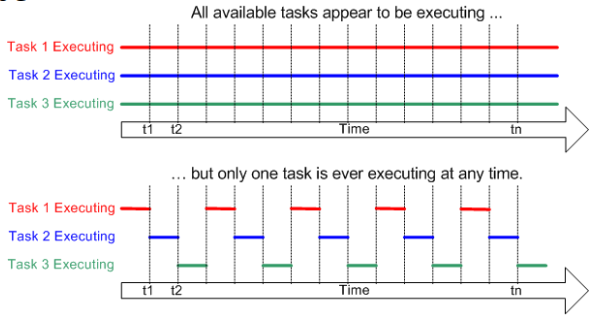
\includegraphics[width=0.6\textwidth]{images/multitasking.png}
\end{center}

\textbf{Scheuler}

The scheduler is a part of the kernel that decides which task will be executed when.
The scheduler can suspend and resume tasks, but tasks can suspend themselves too.
When the scheduler switches between tasks, it is called a context switch.
Tasks use different resources of the microcontroller, such as registers,
stack, and program counter.
When the kernel switches tasks, it saves its context,
and resumes from it once a task is resumed.


\textbf{FreeRTOS choice of scheduling policy}

Two choices: Preemptive and Cooperative. Pre-emptive always runs the highest priority task that is ready to run.
Having multiple tasks with the same priority, they will run using round robin scheduling.
Co-operative scheduling is where context switches only occur if a task blocks or explicitly calls task YIELD().


\textbf{FreeRTOS Task States}

There are four states in FreeRTOS:
Running, Ready, Blocked, Suspended.
Running is the task that is currently executing.
Ready is where the task is able to execute but is not currently executing due to another task with equal or higher priority running.
Blocked is where the task waits for a temporal or external event. It can block waiting for a queue or semaphore event.
Suspended is where the task is not available for scheduling. Tasks only enter or exit suspend by vTaskSuspend() and xTaskResume().

\begin{center}
	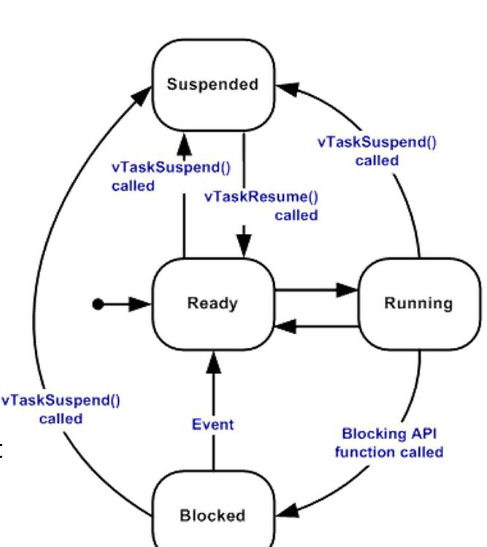
\includegraphics[width=0.4\textwidth]{images/freeStates.png}
\end{center}

\textbf{Additional features of FreeRTOS}

\begin{itemize}
	\item Message Queues: Used for inter-task communication. A task can send a message to a queue and another task can receive it.
	\item Binary and counting semaphores.
	\item Mutexes.
\end{itemize}



\textbf{Sempahores}

Semaphores are used to synchronize tasks and protect shared resources.
A semaphore can be a signaling semaphore or a mutex.
Meaning that a semaphore can be used to signal between tasks or to lock a resource.
Semaphores can be binary or counting.

\textbf{Resource Management}

There is a potential risk for a conflict in a multitasking system. If one task starts to access a resource
but does not complete its access before being transitioned out of the running state. If the task left the resource
in an inconsistent state, then access to the same resource by any other task or interrupt could result in data corruption.

\textbf{Mutual exclusion}

Mutual exclusion can be implemented in FreeRTOS by: Disabling interrupts, using a mutex or disabling the scheduler.

\textbf{Mutex}

A mutex is a special type of binary semaphore that is used to control access to a resource.
Mutex vs. Semaphore: Mutexes can be released only by the task which took them, while binary semaphores can be released
by any task. Mutexes are for protecting resources - binary semaphores are for serialization and signaling.


\textbf{Queues in FreeRTOS}

A queue can hold a finite number of fixed size data items.
The maximum number of items a queue can hold is called its length.
Writing data to a queue causes a byte for byte copy of the data to be
stored in the queue itself. Reading data from a queue causes the
copy of the data to be removed from the queue.


\textbf{Preemption}

The general definition of preemption is a prior seizure
or apporiation - taking possession before others.

A synonym for preemption is protective, defiensive, precautionary.
In computing preemption is the act of temporarily interrupting a task
with the intention of resuming it later.



